\documentclass{standalone}
\usepackage{tikz}
\usepackage{pgfplots}
\usepackage{graphicx}
\usetikzlibrary{positioning,3d,decorations.markings,calc,perspective}
\pgfplotsset{compat=1.18}

\begin{document}
\begin{tikzpicture}[
    x={(0.866cm,-0.5cm)},
    y={(0.866cm,0.5cm)},
    z={(0cm,1cm)}
]
    % Axe temporel
    \draw[->] (0,0,0) -- (12,0,0) node[right] {$t$};
    
    % Points temporels importants
    \draw (8,0,0.1) -- (8,0,-0.1) node[below] {$T=8$};
    \draw (5,0,0.1) -- (5,0,-0.1) node[below] {$t_s$};
    \draw (2,0,0.1) -- (2,0,-0.1) node[below] {$t_c$};
    \draw (0,0,0.1) -- (0,0,-0.1) node[below] {$T=0$};
    
    % Zones de régimes colorées - diviser y par 2
    \fill[blue!20,opacity=0.3] (8,-1,0) -- (8,1,0) -- (5,1,0) -- (5,-1,0) -- cycle; % Régime III
    \fill[green!20,opacity=0.3] (5,-1,0) -- (5,1,0) -- (2,1,0) -- (2,-1,0) -- cycle; % Régime II
    \fill[red!20,opacity=0.3] (2,-1,0) -- (2,1,0) -- (0,1,0) -- (0,-1,0) -- cycle; % Régime I
    
    % Labels des régimes
    \node[above] at (6.5,0,0) {Régime III};
    \node[above] at (3.5,0,0) {Régime II};
    \node[above] at (1,0,0) {Régime I};

    % Définir les styles pour les images en perspective
    \tikzset{
        perspective image/.style={
            canvas is xy plane at z=#1,
            transform shape,
        }
    }

    % Encarts pour les coupes aux extrémités (T=0 et T=8) - tailles divisées par 2
    % T=0 (background)
    \begin{scope}[canvas is yz plane at x=0,on background layer]
        % Rectangle centré sur l'axe temporel
        %\draw[dashed] (-5,-5) rectangle (5,5);
        \node[perspective image=0] at (0,0) {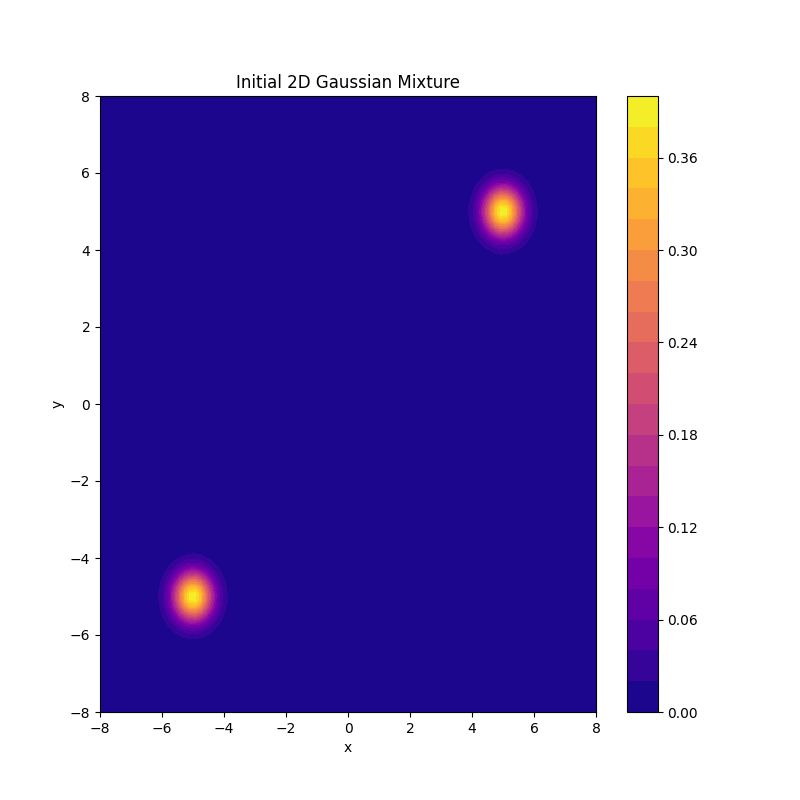
\includegraphics[width=2.5cm,height=1.5cm]{mixture.png}};
    \end{scope}
    % T=8 (background)
    \begin{scope}[canvas is yz plane at x=8,on background layer]
        % Rectangle centré sur l'axe temporel
        %\draw[dashed] (-5,-5) rectangle (5,5);
        \node[perspective image=0] at (0,0) {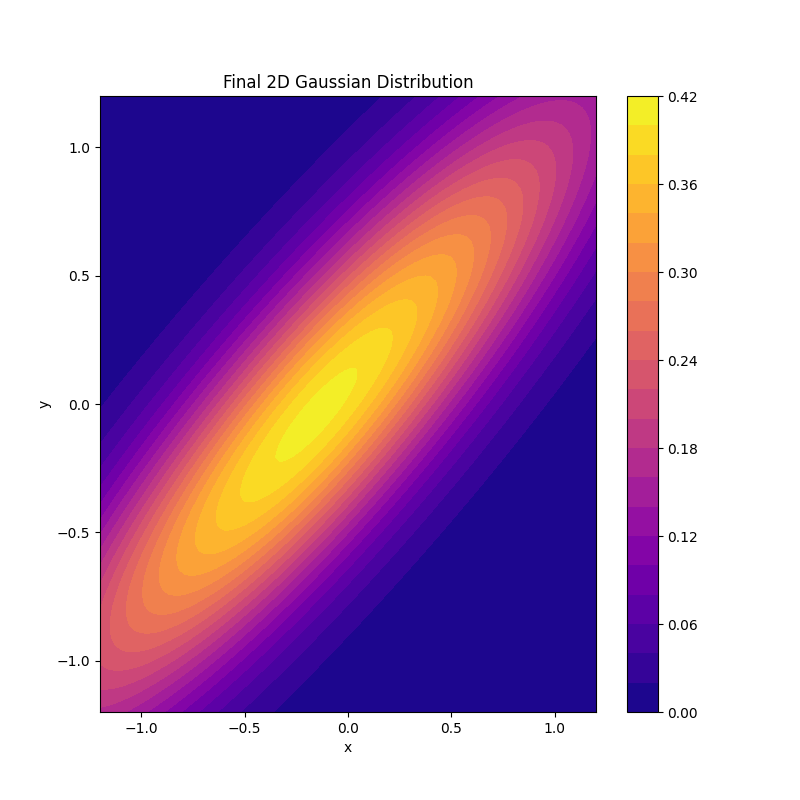
\includegraphics[width=2.5cm,height=2cm,opacity=0.2]{gaussian.png}};
    \end{scope}

    % Encarts pour les coupes (y,z) - diviser les dimensions par 2
    % Régime I - y positif
    \begin{scope}[canvas is yz plane at x=1]
        \draw[dashed] (0,0) rectangle (0.75,1);
        \node[anchor=south west, font=\tiny] at (0.375,1) {$y>0$};
        \node[perspective image=0.5] at (0.375,0.5) {\includegraphics[width=0.65cm,height=0.85cm]{regime1_pos.png}};
    \end{scope}
    
    % Régime I - y négatif
    \begin{scope}[canvas is yz plane at x=1]
        \draw[dashed] (-0.75,0) rectangle (0,1);
        \node[anchor=north west, font=\tiny] at (-0.375,1) {$y<0$};
        \node[perspective image=0.5] at (-0.375,0.5) {\includegraphics[width=0.65cm,height=0.85cm]{regime1_neg.png}};
    \end{scope}
    
    % Régime II - y positif
    \begin{scope}[canvas is yz plane at x=3.5]
        \draw[dashed] (0,0) rectangle (0.75,1);
        \node[anchor=south west, font=\tiny] at (0.375,1) {$y>0$};
        \node[perspective image=0.5] at (0.375,0.5) {\includegraphics[width=0.65cm,height=0.85cm]{regime2_pos.png}};
    \end{scope}
    
    % Régime II - y négatif
    \begin{scope}[canvas is yz plane at x=3.5]
        \draw[dashed] (-0.75,0) rectangle (0,1);
        \node[anchor=north west, font=\tiny] at (-0.375,1) {$y<0$};
        \node[perspective image=0.5] at (-0.375,0.5) {\includegraphics[width=0.65cm,height=0.85cm]{regime2_neg.png}};
    \end{scope}
    
    % Régime III - y positif
    \begin{scope}[canvas is yz plane at x=7]
        \draw[dashed] (0,0) rectangle (0.75,1);
        \node[anchor=south west, font=\tiny] at (0.375,1) {$y>0$};
        \node[perspective image=0.5] at (0.375,0.5) {\includegraphics[width=0.65cm,height=0.85cm]{regime3_pos.png}};
    \end{scope}
    
    % Régime III - y négatif
    \begin{scope}[canvas is yz plane at x=7]
        \draw[dashed] (-0.75,0) rectangle (0,1);
        \node[anchor=north west, font=\tiny] at (-0.375,1) {$y<0$};
        \node[perspective image=0.5] at (-0.375,0.5) {\includegraphics[width=0.65cm,height=0.85cm]{regime3_neg.png}};
    \end{scope}

    % Trajectoire 1 (rouge) - diviser y et z par 2
    \draw[red,opacity=0.4] plot coordinates {
        (0,-0.797,-0.844) (0.08,-0.778,-0.801) (0.16,-0.785,-0.807) (0.24,-0.740,-0.786)
        (0.32,-0.753,-0.770) (0.40,-0.767,-0.784) (0.48,-0.760,-0.838) (0.56,-0.809,-0.854)
        (0.64,-0.837,-0.845) (0.72,-0.863,-0.885) (0.80,-0.821,-0.891) (0.88,-0.819,-0.931)
        (0.96,-0.835,-0.928) (1.04,-0.867,-0.918) (1.12,-0.884,-0.926) (1.20,-0.901,-0.873)
        (1.28,-0.902,-0.903) (1.36,-0.879,-0.938) (1.44,-0.873,-0.993) (1.52,-0.910,-0.988)
        (1.60,-0.889,-0.983) (1.68,-0.893,-0.991) (1.76,-0.934,-1.012) (1.84,-0.947,-0.982)
        (1.92,-0.938,-1.032) (2.00,-0.929,-1.043) (2.08,-0.948,-1.025) (2.16,-0.919,-0.999)
        (2.24,-0.942,-1.008) (2.32,-0.933,-0.980) (2.40,-0.946,-0.985) (2.48,-0.978,-1.019)
        (2.56,-0.955,-0.981) (2.64,-0.957,-0.952) (2.72,-0.947,-0.971) (2.80,-0.936,-0.927)
        (2.88,-0.937,-0.883) (2.96,-1.011,-0.860) (3.04,-1.009,-0.868) (3.12,-1.006,-0.924)
        (3.20,-1.013,-0.914) (3.28,-0.971,-0.929) (3.36,-0.994,-0.943) (3.44,-0.968,-0.934)
        (3.52,-0.983,-0.919) (3.60,-0.980,-0.892) (3.68,-1.000,-0.901) (3.76,-1.011,-0.943)
        (3.84,-1.003,-0.935) (3.92,-1.002,-0.942) (4.00,-1.043,-0.954) (4.08,-1.052,-0.976)
        (4.16,-1.057,-0.965) (4.24,-1.003,-0.960) (4.32,-0.996,-0.962) (4.40,-1.050,-0.963)
        (4.48,-1.049,-0.893) (4.56,-1.054,-0.885) (4.64,-1.055,-0.918) (4.72,-1.023,-0.896)
        (4.80,-1.000,-0.922) (4.88,-0.961,-0.962) (4.96,-0.944,-0.900) (5.04,-0.972,-0.916)
        (5.12,-0.969,-0.930) (5.20,-1.013,-0.928) (5.28,-1.043,-0.915) (5.36,-1.069,-0.871)
        (5.44,-1.091,-0.880) (5.52,-1.068,-0.915) (5.60,-1.062,-0.878) (5.68,-1.107,-0.873)
        (5.76,-1.100,-0.851) (5.84,-1.135,-0.888) (5.92,-1.120,-0.880) (6.00,-1.113,-0.870)
        (6.08,-1.132,-0.863) (6.16,-1.124,-0.883) (6.24,-1.071,-0.870) (6.32,-1.105,-0.851)
        (6.40,-1.133,-0.829) (6.48,-1.100,-0.852) (6.56,-1.073,-0.841) (6.64,-1.049,-0.787)
        (6.72,-1.056,-0.808) (6.80,-1.081,-0.831) (6.88,-1.084,-0.822) (6.96,-1.076,-0.798)
        (7.04,-1.075,-0.757) (7.12,-1.083,-0.680) (7.20,-1.065,-0.705) (7.28,-1.096,-0.691)
        (7.36,-1.102,-0.671) (7.44,-1.088,-0.673) (7.52,-1.112,-0.716) (7.60,-1.125,-0.691)
        (7.68,-1.119,-0.727) (7.76,-1.114,-0.716) (7.84,-1.139,-0.711) (7.92,-1.137,-0.744)
    };

    % Trajectoire 2 (bleu) - diviser y et z par 2
    \draw[blue,opacity=0.4] plot coordinates {
        (0,-0.807,-0.792) (0.08,-0.776,-0.762) (0.16,-0.815,-0.789) (0.24,-0.801,-0.774)
        (0.32,-0.786,-0.665) (0.40,-0.770,-0.633) (0.48,-0.743,-0.614) (0.56,-0.752,-0.593)
        (0.64,-0.774,-0.600) (0.72,-0.787,-0.597) (0.80,-0.722,-0.650) (0.88,-0.703,-0.696)
        (0.96,-0.716,-0.665) (1.04,-0.714,-0.695) (1.12,-0.734,-0.676) (1.20,-0.755,-0.670)
        (1.28,-0.754,-0.689) (1.36,-0.693,-0.671) (1.44,-0.750,-0.665) (1.52,-0.769,-0.641)
        (1.60,-0.792,-0.645) (1.68,-0.777,-0.620) (1.76,-0.811,-0.629) (1.84,-0.825,-0.648)
        (1.92,-0.775,-0.637) (2.00,-0.810,-0.611) (2.08,-0.750,-0.581) (2.16,-0.793,-0.595)
        (2.24,-0.757,-0.615) (2.32,-0.745,-0.593) (2.40,-0.771,-0.595) (2.48,-0.863,-0.624)
        (2.56,-0.870,-0.659) (2.64,-0.824,-0.700) (2.72,-0.836,-0.696) (2.80,-0.795,-0.736)
        (2.88,-0.763,-0.736) (2.96,-0.790,-0.723) (3.04,-0.785,-0.740) (3.12,-0.783,-0.751)
        (3.20,-0.779,-0.732) (3.28,-0.735,-0.767) (3.36,-0.674,-0.822) (3.44,-0.679,-0.806)
        (3.52,-0.671,-0.823) (3.60,-0.677,-0.837) (3.68,-0.693,-0.813) (3.76,-0.683,-0.833)
        (3.84,-0.658,-0.824) (3.92,-0.635,-0.806) (4.00,-0.658,-0.822) (4.08,-0.637,-0.805)
        (4.16,-0.638,-0.802) (4.24,-0.601,-0.818) (4.32,-0.586,-0.824) (4.40,-0.592,-0.793)
        (4.48,-0.569,-0.770) (4.56,-0.532,-0.769) (4.64,-0.513,-0.778) (4.72,-0.503,-0.782)
        (4.80,-0.501,-0.765) (4.88,-0.524,-0.706) (4.96,-0.552,-0.740) (5.04,-0.519,-0.718)
        (5.12,-0.502,-0.700) (5.20,-0.502,-0.725) (5.28,-0.500,-0.745) (5.36,-0.472,-0.749)
        (5.44,-0.496,-0.758) (5.52,-0.484,-0.774) (5.60,-0.507,-0.767) (5.68,-0.500,-0.781)
        (5.76,-0.514,-0.775) (5.84,-0.555,-0.815) (5.92,-0.575,-0.821) (6.00,-0.566,-0.779)
        (6.08,-0.542,-0.783) (6.16,-0.543,-0.812) (6.24,-0.543,-0.820) (6.32,-0.534,-0.843)
        (6.40,-0.519,-0.800) (6.48,-0.522,-0.789) (6.56,-0.503,-0.800) (6.64,-0.496,-0.800)
        (6.72,-0.494,-0.821) (6.80,-0.493,-0.807) (6.88,-0.452,-0.780) (6.96,-0.391,-0.802)
        (7.04,-0.366,-0.797) (7.12,-0.304,-0.820) (7.20,-0.328,-0.837) (7.28,-0.388,-0.851)
        (7.36,-0.410,-0.847) (7.44,-0.400,-0.794) (7.52,-0.373,-0.810) (7.60,-0.399,-0.796)
        (7.68,-0.436,-0.745) (7.76,-0.403,-0.758) (7.84,-0.451,-0.720) (7.92,-0.454,-0.685)
    };

    % Trajectoire 3 (vert) - diviser y et z par 2
    \draw[green,opacity=0.4] plot coordinates {
        (0,0.715,0.789) (0.08,0.715,0.790) (0.16,0.702,0.808) (0.24,0.672,0.804)
        (0.32,0.675,0.818) (0.40,0.695,0.787) (0.48,0.652,0.823) (0.56,0.662,0.802)
        (0.64,0.705,0.805) (0.72,0.739,0.807) (0.80,0.797,0.856) (0.88,0.790,0.884)
        (0.96,0.808,0.923) (1.04,0.781,0.942) (1.12,0.811,0.892) (1.20,0.777,0.835)
        (1.28,0.770,0.855) (1.36,0.812,0.857) (1.44,0.858,0.818) (1.52,0.810,0.816)
        (1.60,0.821,0.815) (1.68,0.763,0.813) (1.76,0.726,0.832) (1.84,0.736,0.805)
        (1.92,0.721,0.775) (2.00,0.720,0.802) (2.08,0.692,0.817) (2.16,0.677,0.794)
        (2.24,0.674,0.765) (2.32,0.658,0.731) (2.40,0.714,0.732) (2.48,0.694,0.738)
        (2.56,0.691,0.732) (2.64,0.708,0.753) (2.72,0.693,0.737) (2.80,0.685,0.672)
        (2.88,0.642,0.710) (2.96,0.689,0.703) (3.04,0.705,0.712) (3.12,0.792,0.744)
        (3.20,0.789,0.717) (3.28,0.743,0.723) (3.36,0.722,0.682) (3.44,0.704,0.652)
        (3.52,0.751,0.677) (3.60,0.751,0.719) (3.68,0.753,0.694) (3.76,0.796,0.709)
        (3.84,0.767,0.704) (3.92,0.742,0.665) (4.00,0.769,0.719) (4.08,0.729,0.735)
        (4.16,0.711,0.721) (4.24,0.694,0.697) (4.32,0.695,0.673) (4.40,0.703,0.672)
        (4.48,0.696,0.646) (4.56,0.680,0.667) (4.64,0.694,0.640) (4.72,0.697,0.661)
        (4.80,0.650,0.676) (4.88,0.631,0.693) (4.96,0.609,0.642) (5.04,0.563,0.643)
        (5.12,0.570,0.617) (5.20,0.589,0.570) (5.28,0.587,0.536) (5.36,0.568,0.537)
        (5.44,0.544,0.527) (5.52,0.572,0.510) (5.60,0.596,0.478) (5.68,0.611,0.519)
        (5.76,0.541,0.496) (5.84,0.557,0.491) (5.92,0.568,0.474) (6.00,0.570,0.469)
        (6.08,0.603,0.476) (6.16,0.613,0.465) (6.24,0.599,0.453) (6.32,0.610,0.441)
        (6.40,0.619,0.499) (6.48,0.643,0.490) (6.56,0.677,0.479) (6.64,0.619,0.450)
        (6.72,0.567,0.440) (6.80,0.567,0.488) (6.88,0.576,0.481) (6.96,0.600,0.419)
        (7.04,0.606,0.441) (7.12,0.565,0.473) (7.20,0.574,0.461) (7.28,0.592,0.525)
        (7.36,0.597,0.532) (7.44,0.584,0.508) (7.52,0.608,0.484) (7.60,0.610,0.471)
        (7.68,0.623,0.480) (7.76,0.653,0.466) (7.84,0.645,0.438) (7.92,0.632,0.449)
    };

    % Trajectoire 4 (violet) - diviser y et z par 2
    \draw[violet,opacity=0.4] plot coordinates {
        (0,0.890,0.765) (0.08,0.915,0.803) (0.16,0.926,0.856) (0.24,0.904,0.821)
        (0.32,0.854,0.863) (0.40,0.873,0.862) (0.48,0.881,0.830) (0.56,0.950,0.834)
        (0.64,0.953,0.854) (0.72,0.966,0.860) (0.80,0.944,0.874) (0.88,0.997,0.912)
        (0.96,1.042,0.897) (1.04,1.014,0.894) (1.12,1.016,0.925) (1.20,0.968,0.968)
        (1.28,0.964,0.956) (1.36,0.935,0.909) (1.44,0.958,0.911) (1.52,0.922,0.875)
        (1.60,0.912,0.922) (1.68,0.905,0.879) (1.76,0.898,0.872) (1.84,0.822,0.870)
        (1.92,0.815,0.890) (2.00,0.867,0.922) (2.08,0.860,0.890) (2.16,0.933,0.892)
        (2.24,0.933,0.891) (2.32,0.939,0.887) (2.40,0.922,0.872) (2.48,0.921,0.856)
        (2.56,0.901,0.859) (2.64,0.894,0.902) (2.72,0.819,0.933) (2.80,0.854,0.874)
        (2.88,0.845,0.864) (2.96,0.805,0.842) (3.04,0.773,0.891) (3.12,0.800,0.927)
        (3.20,0.820,0.895) (3.28,0.805,0.909) (3.36,0.771,0.929) (3.44,0.764,0.919)
        (3.52,0.784,0.931) (3.60,0.774,0.964) (3.68,0.743,0.981) (3.76,0.760,0.973)
        (3.84,0.769,0.937) (3.92,0.796,0.932) (4.00,0.781,0.962) (4.08,0.761,0.922)
        (4.16,0.717,0.939) (4.24,0.681,0.989) (4.32,0.622,1.037) (4.40,0.628,1.034)
        (4.48,0.612,1.045) (4.56,0.611,1.076) (4.64,0.614,1.081) (4.72,0.604,1.079)
        (4.80,0.613,1.031) (4.88,0.575,1.052) (4.96,0.580,1.047) (5.04,0.580,1.056)
        (5.12,0.565,1.034) (5.20,0.570,1.007) (5.28,0.582,0.959) (5.36,0.611,0.972)
        (5.44,0.618,1.000) (5.52,0.665,1.028) (5.60,0.613,0.992) (5.68,0.596,0.993)
        (5.76,0.610,0.972) (5.84,0.616,0.951) (5.92,0.598,0.911) (6.00,0.572,0.873)
        (6.08,0.545,0.903) (6.16,0.518,0.977) (6.24,0.532,0.982) (6.32,0.507,1.002)
        (6.40,0.491,1.006) (6.48,0.564,1.003) (6.56,0.596,0.983) (6.64,0.595,1.033)
        (6.72,0.577,1.084) (6.80,0.597,1.069) (6.88,0.615,1.096) (6.96,0.633,1.052)
        (7.04,0.612,1.045) (7.12,0.610,1.062) (7.20,0.615,1.024) (7.28,0.626,1.042)
        (7.36,0.642,1.072) (7.44,0.665,1.085) (7.52,0.663,1.038) (7.60,0.675,1.044)
        (7.68,0.683,1.008) (7.76,0.653,1.038) (7.84,0.651,1.057) (7.92,0.652,1.058)
    };

    % Légende pour expliquer les sections
    \node[anchor=south east, align=left, font=\scriptsize] at (11,2.5,1) {
        \textbf{Temps critiques:}\\
        $T=0$: Distribution initiale (mélange)\\
        $t_c$: Temps critique de collapse\\
        $t_s$: Temps critique de séparation\\
        $T=8$: Distribution finale (gaussienne)
    };

\end{tikzpicture}
\end{document}
